\documentclass[a4paper,12pt,twoside]{report}
\usepackage[left=1.25in,right=1in,top=2.5in,bottom=1in]{geometry}
\usepackage{graphicx}
%\usepackage[backend=biber,style=apa,maxcitenames=1,natbib=true]{biblatex}
%\addbibresource{References.bib}
\usepackage{enumerate}
\usepackage{emptypage}
\usepackage{pdfpages}
\usepackage{listings}
\renewcommand{\baselinestretch}{1.5}
\usepackage{amsmath}

\newtheorem{defn}{Definitions}
\newtheorem{thm}{Theorem}[section]
\newtheorem{lem}{Lemma}[section]
\newtheorem{cor}{Corollary}[section]

\begin{document}
  \begin{titlepage}
  \begin{center}
    \LARGE
    \textbf{Moran Model}

    \vspace{1.5cm}
    \Large
    \textbf{Manu M.}

    \vfill
    \Large
    \textit{A dissertation submitted for the partial fulfilment of\\
    BS-MS dual degree in Science}

    \vspace{0.8cm}

    
\includegraphics[width=0.3\textwidth]{C0/Figs/IISER_Mohali_logo.png}

    \large
    \textbf{Indian Institute of Science Education and Research, Mohali}\\
    \large
    \textbf{April 2020}
  \end{center}
\end{titlepage}

  \pagenumbering{roman}
  \newgeometry{left=0in,right=0in,top=0in,bottom=1in}
  \addcontentsline{toc}{chapter}{Certificate of Examination}
  \begin{center}
  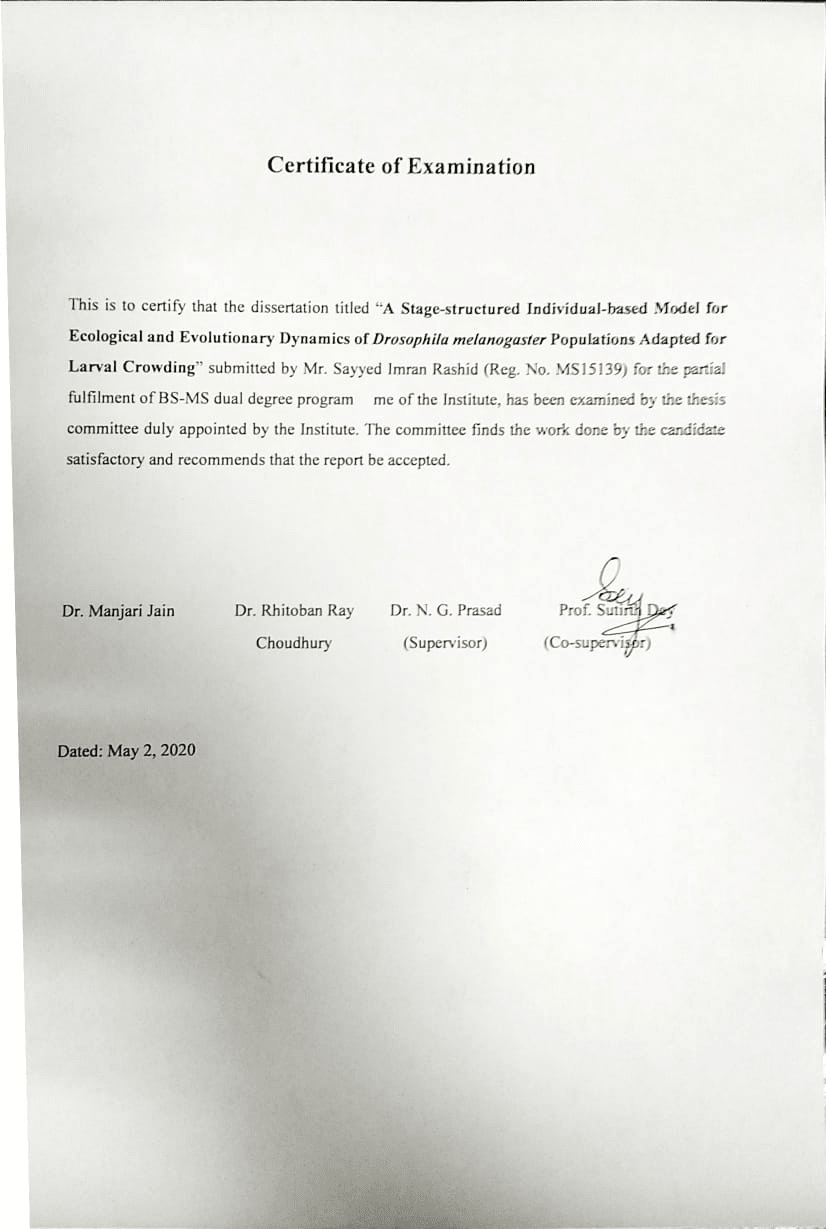
\includegraphics[height=0.9\paperheight, trim= 30 100 70 0, clip ]{C0/Certificate.png}  
\end{center}
\cleardoublepage


  \addcontentsline{toc}{chapter}{Declaration}
  \begin{center}
  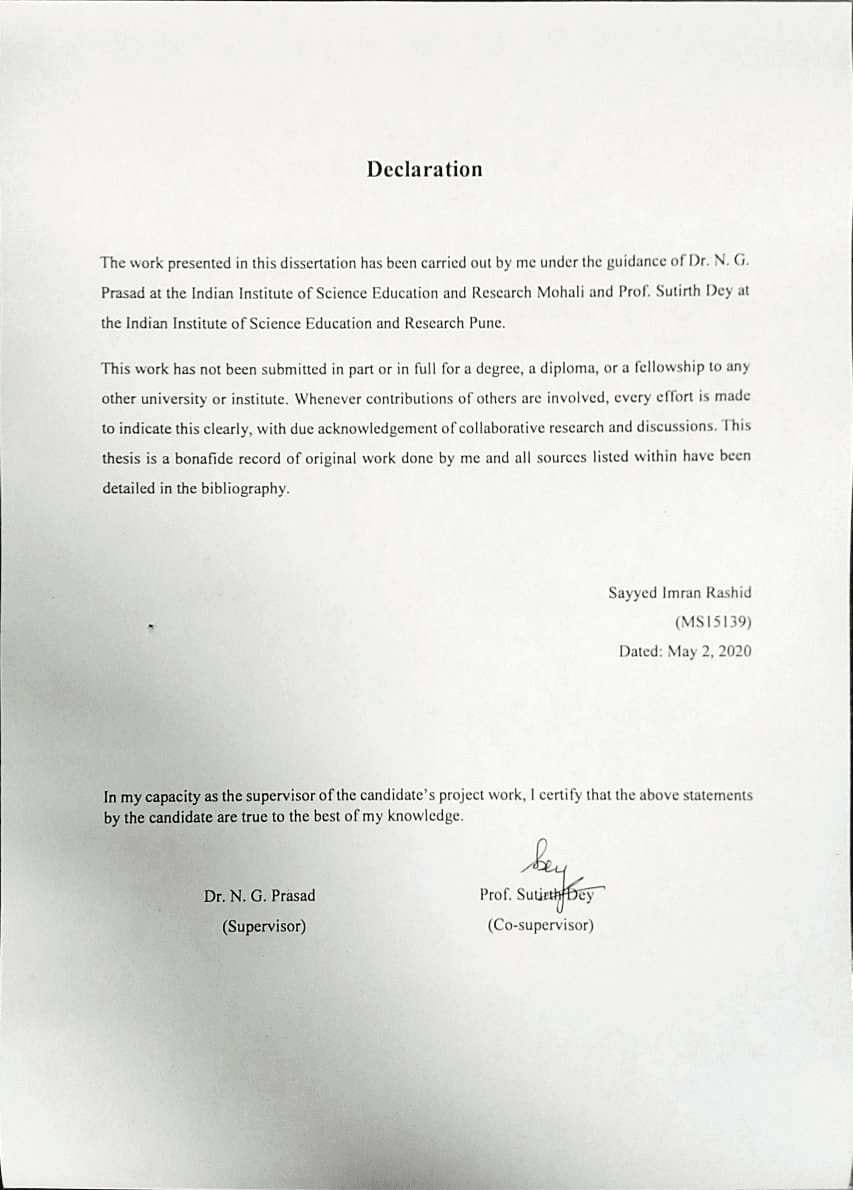
\includegraphics[height=0.9\paperheight, trim= 40 100 60 0, clip ]{C0/Declaration.png}  
\end{center}
\cleardoublepage


  \newgeometry{left=1.25in,right=1in,top=2.5in,bottom=1in}
  \addcontentsline{toc}{chapter}{Acknowledgements}
  \begin{center}
\Large  {\bf Acknowledgements }
\end{center}
I would like to thank Dr. N. G. Prasad and Prof. Sutirth Dey for giving me tremendous support, guidance along with full freedom to work on this thesis. \\\ \
I wish to acknowledge the committee members Dr. Manjari Jain and Dr. Rhitoabn Ray Choudhury for their suggestions and timely review of the progress of my work.\\\\
I am thankful to Dr. Sudipta Tung for introducing me to this project in the first place and guiding me through the beauty of the simulation work. I am extremely grateful for all his encouragement and suggestions for starting this work.\\\\
I am also thankful to Prof. Amitabh Joshi for giving helpful suggestions to my work along with great encouragements. I am grateful to people in EBL and PBL for their constant support, inputs, discussions and fun.\\\\
I would also like to thank all of my friends making life amazing at each moment. I am also grateful to $7^{th}$ floor productions for all kinds of memories.\\\\
I further extend my gratitude towards Dr. N. G. Prasad, who helped me at any step needed, guided me through difficult situations. I am grateful to him for being an excellent mentor.\\\\
Finally, I especially thank my parents and my sisters for being incredibly supportive and encouraging me during my work.
\vfill
\cleardoublepage


  \newgeometry{left=1.25in,right=1in,top=1in,bottom=1in}

  \addcontentsline{toc}{chapter}{List of Figures}
  \listoffigures

  \addcontentsline{toc}{chapter}{List of Tables}
  \listoftables

  \setcounter{tocdepth}{1}
  \tableofcontents

  \addcontentsline{toc}{chapter}{Abstract}

\begin{abstract}

\lipsum

\end{abstract}


  \pagenumbering{arabic}
  \chapter{Introduction}
The theory of density-dependent natural selection was verbally introduced by \citet{macarthurGENERALIZEDTHEOREMSNATURAL1962}, \citet*{macarthurTheoryIslandBiogeography1967} to explore the evolution of phenotypes dependent on the population density. It is considered to be a critical link between ecological and evolutionary dynamics \citep{muellerTheoreticalEmpiricalExamination1997}. Over many years, this theory has been modified mathematically and studied experimentally to understand density effects on the evolution in great detail \citep{andersonDensityRegulatedSelectionGenotypic1983,asmussenDensityDependentSelectionIncorporating1983,clarkeDensityDependentSelection1972,muellerTheoreticalEmpiricalExamination1997,roughgardenDensityDependentNaturalSelection1971,santosDensityDependentNaturalSelection1997}. Early experimental studies also showed that selection at extreme densities causes selection for higher competitive ability since there is competition for limited resources \citep{joshiKselectionAselectionEffectiveness2001}. Such competitive ability of an organism is composite phenotype determined by various life-history traits. Through these early studies, it was clear that density is a significant factor in determining the life-history of organisms which are essential for competitive ability. Competition plays a vital role in determining not only evolutionary outcomes of species but also ecological outcomes which affect population dynamics and interactions with other species \citep{caseIllustratedGuideTheoretical2000a,deyAdaptationLarvalCrowding2012}. Thus, in order to grasp a better understanding of density-dependent selection, exploring the effect of competitive ability on ecological and evolutionary dynamics becomes essential \citep{prasadWhatHaveTwo2003}.  \\\\
Over the last four decades, various \textit{Drosophila melanogaster} laboratory populations have been used to study the evolution of life-history traits due to density-dependent selection. One of the first experimental evolution studies used r and \textit{K}-selected populations of \textit{Drosophila melanogaster} \citep{muellerTradeoffRselectionKselection1981} ) to investigate the \textit{r}- and \textit{K}-selection theory by  \citet{macarthurGENERALIZEDTHEOREMSNATURAL1962}, \citet*{macarthurTheoryIslandBiogeography1967}. In these populations, \textit{r}-selection lines were maintained at low-density, giving density-independent selection. In contrast, lines for \textit{K}-selection were maintained at extreme densities such that selection was density-dependent. As predicted by early mathematical models, these studies showed that \textit{r}-selected populations favoured traits responsible for highe\textit{r}-selected population growth rate at low densities but lower growth rate at extreme density. \citet{bakkerAnalysisFactorsWhich1962,burnetGeneticAnalysisLarval1977} suggested that larval feeding rate, which is measured as retraction rate of cephalopharyngeal sclerites of the larva, is a critical factor in larval competitive ability. Experimental studies on \textit{r}- and \textit{K}-selection showed that \textit{K}-selected populations have higher competitive ability along with increased larval feeding rate \citep{joshiEvolutionHigherFeeding1988}. This led to the conclusion that larval feeding rate is a good measure of competitive ability in \textit{Drosophila} larvae. These populations could not predict classical density-dependent outcomes such as higher efficiency of food into biomass conversion \citep{muellerDensitydependentNaturalSelection1990}. Another problem with these populations was that \textit{r}-selected populations were maintained in discrete generation cycles while \textit{K}-selected populations were maintained in overlapping generations. \\\\
The successive experimental evolution studies were aimed at tackling questions raised in experimental studies mentioned above, by having a stage-specific density-dependent selection in a new set of \textit{D. melanogaster} populations (described in \cite{joshiDirectionalStabilizingDensityDependent1993}). In this long-term evolution study, a set of larval crowding (CU) population, another set of adult crowding (UC) population and one set of uncrowded (UU) \textit{D. melanogaster} population were used. CU population adapted to larval crowding through a similar set of traits seen in \textit{K}-selected populations. CU population had higher competitive ability than UU population at high-density which leads to increased pre-adult survivorship and decreased pre-adult development time \citep{borashPatternsSelectionStress2001,joshiDirectionalStabilizingDensityDependent1993,santosDensityDependentNaturalSelection1997}. Such competitive ability in CU larvae was due to increased feeding rate and increased nitrogenous waste tolerance at the cost of poor efficiency to convert food into biomass \citep{borashGeneticPolymorphismMaintained1998,joshiDensitydependentNaturalSelection1996,shiotsuguSymmetryCorrelatedSelection1997}. These results established a canonical view of density-dependent selection in \textit{Drosophila} which argued that the evolution of greater competitive ability occured through increased feeding rate and metabolic waste tolerance at the cost of efficiency of food utilization \citep{joshiKselectionAselectionEffectiveness2001}. \\\\
After the canonical view on adaptation to larval crowding was accepted widely, recent studies in different \textit{Drosophila} species questioned this view. A subsequent study on adaptation to larval crowding involved \textit{D. ananassae} and \textit{D. nasuta nasuta} species of \textit{Drosophila} which were wild-caught and subjected to long-term selection experiments similar to UU-CU populations \citep{nagarajanAdaptationLarvalCrowding2016}. Unlike CU population these were maintained at similar larval density but with decreased absolute number of eggs and total larval food. Due to adaptation to larval crowding in these populations, there was an increase in pre-adult survivorship at high-density and faster development compared to control at both low and high-density. In contrast to results from previous K and CU populations, these populations showed a reduction in time to reach critical size with no increase in larval feeding rate nor in nitrogenous waste tolerance \citep{nagarajanAdaptationLarvalCrowding2016}. Such reduced minimum critical feeding time was speculated to be due to increased efficiency of food into biomass conversion, which fit the \textit{K}-selection theory of \citet*{macarthurTheoryIslandBiogeography1967}. These surprising results were thought to be an outcome of several factors such as differences in species-specific genetic architect of traits responsible for larval competitive ability, differences in wild-caught populations and long-term laboratory populations, as well as differences in maintains of larval crowding suggesting the effect of ecological factors.\\\\
A  long-term follow-up study on adaptation to larval crowding was performed using \textit{Drosophila melanogaster} populations derived from UU populations to answer the questions raised from larval crowding studies of \citet{nagarajanAdaptationLarvalCrowding2016}. In this study, a set of control  populations (MB: Melanogaster Baseline) which had low larval density, and another set of populations (MCU: Melanogaster Crowded as larvae Uncrowded as adults) where larval stage was maintained at high-density similar to larval crowded populations of \textit{D. ananassae} and \textit{D. nasuta nasuta} \citep{sarangiEvolutionIncreasedLarval2016}. MCU population showed the evolution of greater larval competitive ability through a similar set of traits observed in the study of \citet{nagarajanAdaptationLarvalCrowding2016}, i.e. decrease in the time to reach critical size without an increase in feeding rate. MCU larvae also did not differ in terms of metabolic waste tolerance but still showed faster pre-adult development time at both densities \citep{sarangiEvolutionIncreasedLarval2016}. In addition to these results, both MB and MCU populations showed a significant lower survivorship in the larval density of 1200 eggs / 6 ml food (CU-type culture) than in larval density of 600 eggs / 1.5 ml food (MCU-type culture) \citep{sarangiPreliminaryInvestigationsCauses2013}. MCU and CU population were derived from the same ancestry but still showed differences, indicating that ecological factors such as the overall number of eggs and total larval food, would be playing a significant role in determining which traits are selected for achieving greater competitive ability under larval crowding. \\\\
A subsequent study exploring ecological factors affecting adaptation to larval crowding involved two new set \textit{D. melanogaster} populations derived from MB population. One set of these populations was CCU (Control Crowded as larvae Uncrowded as adults) population to address the effect of the absolute number of eggs and total food on evolution od larval competitive ability. Another set of populations was LCU (Larry Mueller Crowded as larvae Uncrowded as adults) population aimed at controlling for the food differences between CU and MCU populations since larval food used in these populations were banana and cornmeal medium respectively. In all these four \textit{D. melanogaster} populations (MB, MCU, CCU and LCU) the adult stage was maintained in pretty much similar manner, whereas the details of larval stage maintenance are given in table~\ref{tab:larval_pop} \citep{sarangiEcologicalDetailsMediate2018}.
\begin{table}[h]
  \centering
  \begin{tabular}{|c|c|c|c|c|}
    \hline
    \textbf{No.} & \textbf{Population} & \textbf{No. of eggs} & \textbf{Food volume} & \textbf{Vial dimensions} \\
    \hline
    1. & MB & 70 & 6 ml & 9.5 cm \textit{h} $\times$ 2.4 cm \textit{d} \\
    \hline
    2. & MCU & 600 & 1.5 ml & 9.5 cm \textit{h} $\times$ 2.4 cm \textit{d} \\
    \hline
    3. & CCU & 1200 & 3 ml & 9.5 cm \textit{h} $\times$ 2.4 cm \textit{d} \\
    \hline
    4. & LCU & 1200 & 6 ml & 9.5 cm \textit{h} $\times$ 2.2 cm \textit{d} \\
    \hline
  \end{tabular}
  \caption{Larval stage maintenance in MB, MCU, CCU and LCU populations}
  \label{tab:larval_pop}
\end{table}\\
After several generations of selection, CCU and LCU populations showed an increase in competitive ability and had higher pre-adult survivorship compared to MB population at high densities \citep{sarangiEcologicalDetailsMediate2018}. These two populations showed much higher feeding rate along with no difference in nitrogenous waste tolerance for achieving greater competitive ability, unlike MCU population. These results were interesting since MCU and CCU populations were maintained at the same larval density with varying total number of eggs and food. \citet{sarangiEcologicalDetailsMediate2018} also showed that feeding rate measured at the third instar stage of these larvae was dependent on the number of larvae present during larval feeding when assayed in slial (slide vials) treatment. When assayed inside culture vials, it was observed that the overall feeding rate of MCU population was the highest in all three high-density treatments in contrast to previous results performed on petri-dish. This result suggested that the ecological dynamics of the culture vial does play an essential role in determining competitive ability.\\\\
Inside a culture vial, larval feeding occurs only at the topmost part of total food present due to their inability to dig more \citep{godoy-herreraInterIntrapopulationalVariation1977}. The available upper part of the total food is approx 1 cm in the height of a standard vial used in MB, MCU and CCU populations, and is
called as 'feeding band' \citep{sarangiEcologicalDetailsMediate2018}. Thus, the sufficient larval density, i.e. number of larvae per feeding band is double in CCU population than in MCU population. Another significant finding regarding ecological dynamics inside a culture vial was the diffusion of metabolic waste excreted by larvae from the feeding band into the food below \citep{sarangiEcologicalDetailsMediate2018}. In MCU culture vials, the total amount of food is almost similar to the size of the feeding band. This lead to the speculation that in MCU culture vial, there is little-to-no diffusion of metabolic waste from the feeding band and food quality may decrease very rapidly during larval feeding affecting competitive ability. In CCU and LCU culture vials, diffusion of such metabolic waste occurs from the feeding band which leads could lead to a slower decrease in food quality affecting competitive ability in a manner different than in MCU culture vial.\\\\
In MCU, CCU and LCU populations, apart from pre-adult survivorship and feeding rate, other life-history traits such as dry weight at eclosion, development time also evolved differently \citep{sarangiEcologicalDetailsMediate2018}. Experimental studies are limiting in order to understand above-mentioned ecological factors inside culture vials of these populations. Thus, a computational simulation approach can be helpful to delve into ecological and evolutionary dynamics in these \textit{Drosophila} populations. \\\\
In this thesis, I have presented a precursory stage-structured individual-based model to investigate adaptation to larval crowding in different crowding conditions based on the study of \citet{sarangiEcologicalDetailsMediate2018}. This model is aimed at linking various ecological factors inside a culture vial, with the evolution of fitness-related traits and greater competitive ability through a combination of various larval traits. The later part of the model is also used to explore the role of initial standing variation in the population as well as heritability of larval traits, in determining the evolutionary trajectories to achieve greater competitive ability. \\\\
\pagebreak


  \chapter{Modelling Larval Stage in a Vial}
 Competition for food during larval stage is determined by not only larval density but also ecological factors inside a food vial such as nitrogenous waste build up (ref), diffusion of waste in the food below (ref), total food amount (ref). Thus, in order to investigate the adaptation to larval crowding, it is crucial to understand the ecology of the vial in which larval stage of Drosophila lab populations is maintained and replicating such environment during larval feeding becomes the first step in modelling the larval growth. Previous experimental studies on Drosophila in laboratory conditions, have shown the pattern of the growth of larvae, excretion of nitrogenous waste, larval feeding behavior in response to the waste excreted, development time (ref). Based on these experimental studies, I have created an individual-based model which considers feeding rate, efficiency to convert food into biomass, critical size and waste tolerance as larval trait parameters to measure other traits which are variables such body size, development time, and survivorship.
\section{Ecology of a Vial in Drosophila Cultures}
During larval feeding inside a vial, larvae are able to access only a certain amount of food from the total food available at a given time point. This is due to their inability to dig more to access food (ref), and this accessible food is referred as the feeding band. For simplicity, feeding band is taken as volume of food proportional to the diameter of the vial. In the model, I also assume this feeding band to be a constant volume of food in all types of culture vials till it reaches the bottom of the vial. The growth of larvae in the model is affected by waste build up and food quality in the feeding band. I also consider a diffusion band which is a part of the total food below feeding band where some amount of waste can diffuse from feeding band at each time step. Fig ~\ref{fig:vial} is the visualization of feeding band and diffusion band during larval feeding.

\begin{figure}[h]
  \centering
  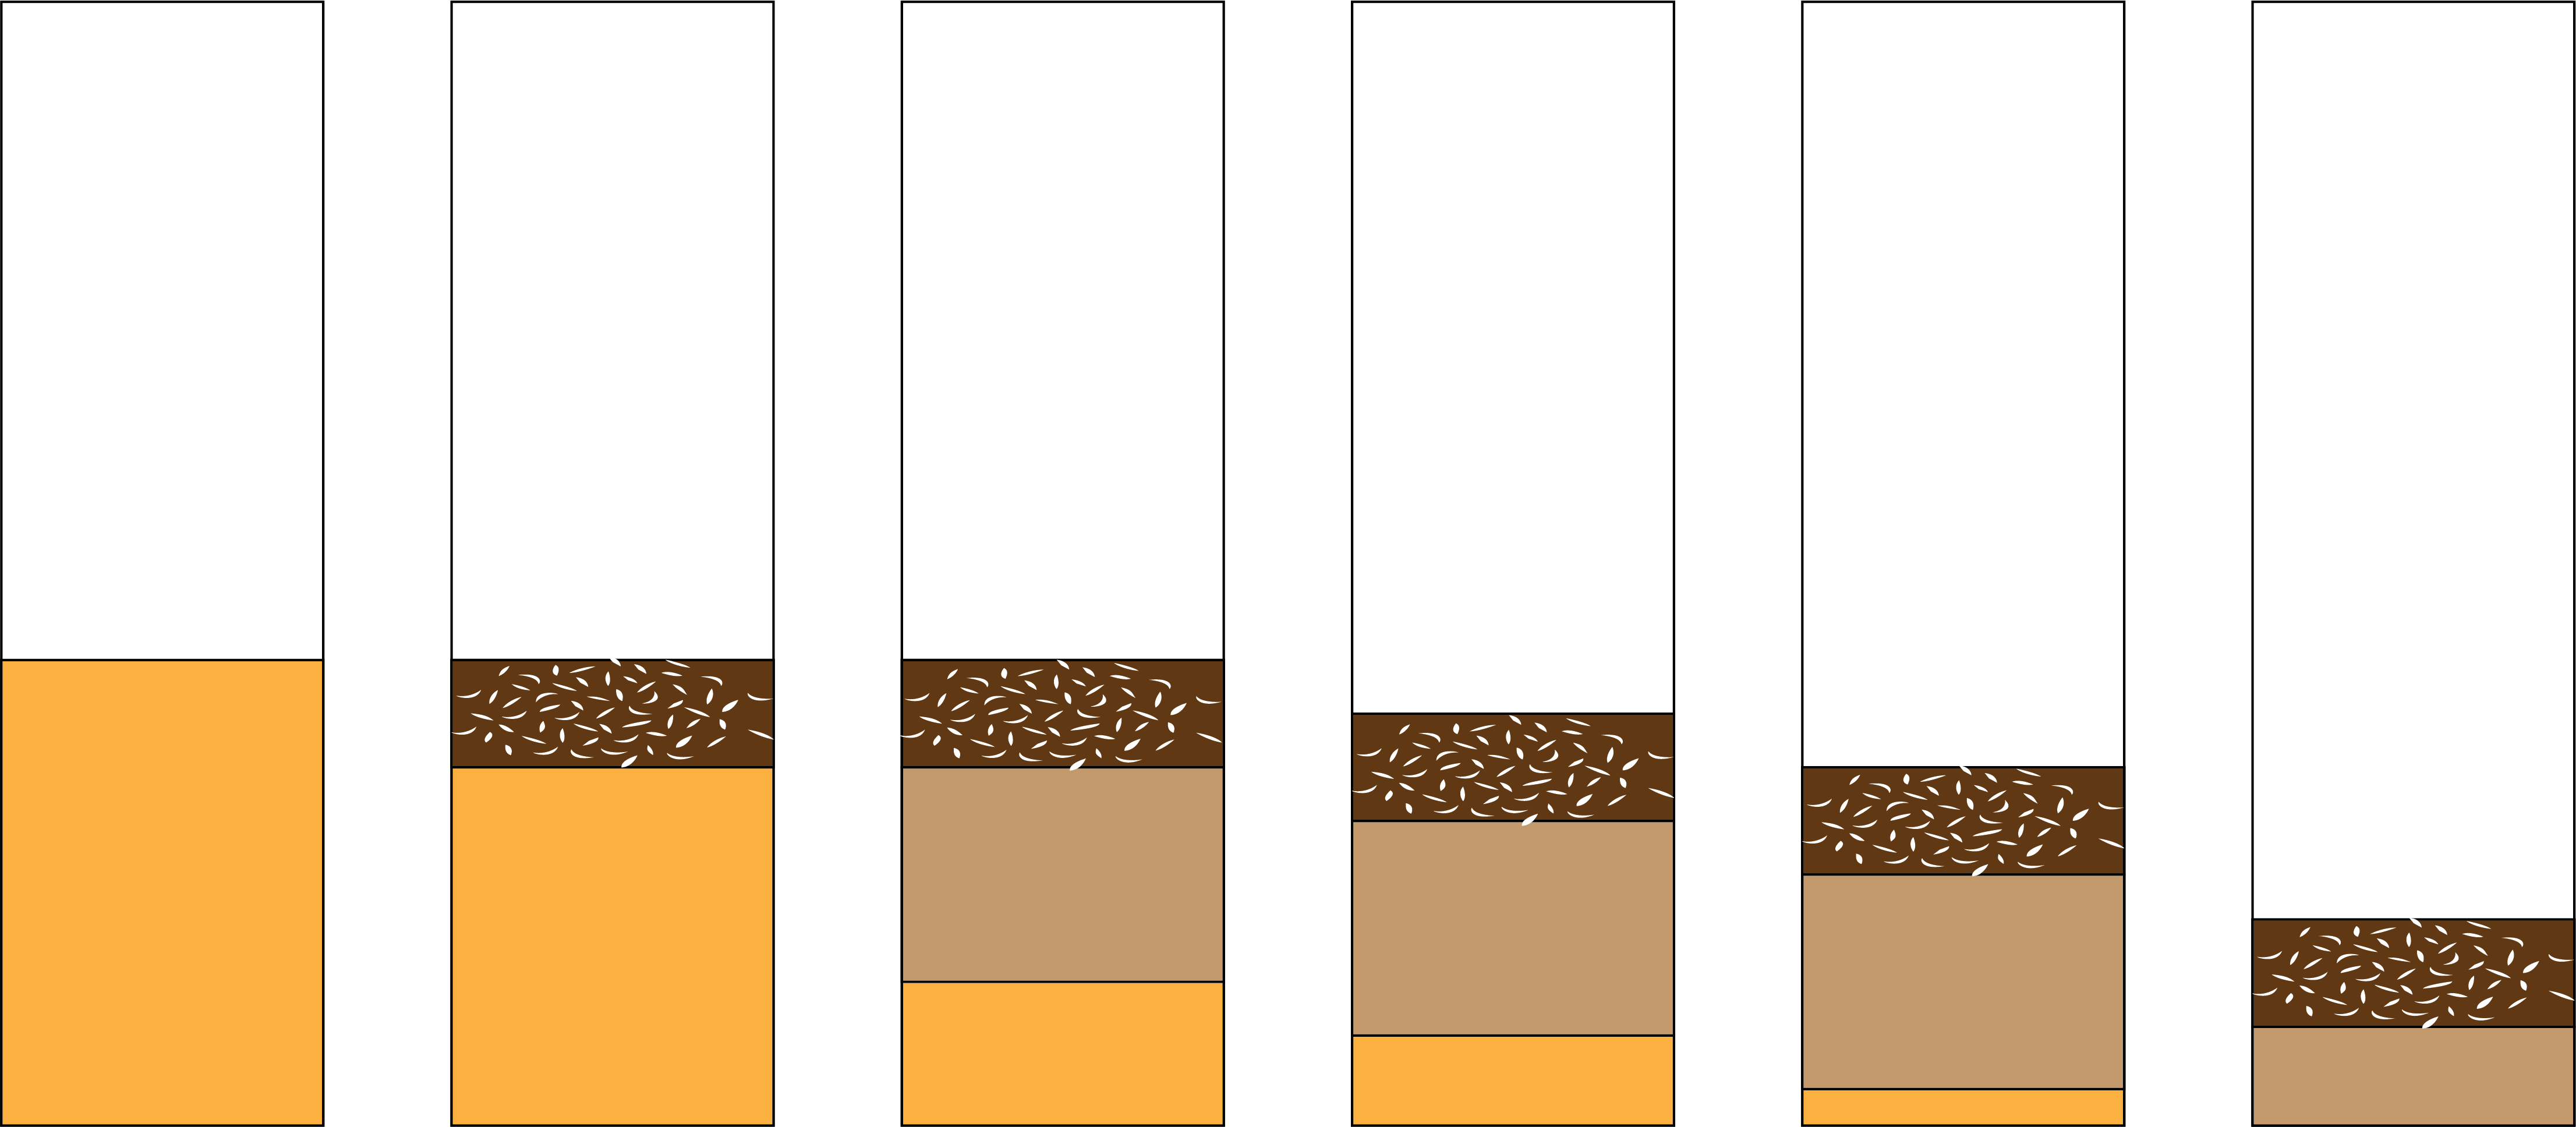
\includegraphics[width=0.75\textwidth]{C2/Figs/vial_diagram}
  \caption{Ecological dynamics in a vial during larval feeding}
  \label{fig:vial}
\end{figure}

\section{Larval Stage Model}
Each individual egg is assigned larval trait parameters from respective distributions with certain mean and variation (table no.). For a given amount of food and number of eggs keeping the sex ratio 1:1, the model follows certain set of rules as described in fig ~\ref{fig:larval_model} which are simulated in discrete time steps. Critical size and efficiency are taken as sexually dimorphic traits and are assigned depending on the sex of the individual larva. Critical size and efficiency of females are assumed to be higher than that of males.\\ \\
The inital size of all larvae is same and the growth is determined by larval trait parameters such as initial feeding rate, efficiency, waste tolerance and critical size assigned to each individual from distributions with respective mean trait value and variation. The larval growth is divided into two stages determined by whether critical size is reached or not, These stages are called pre-critical and post-critical stage. \\
In pre-critical stage of the larva, feeding rate is a linear function of time, given as:
\[Fr_{i}(t) = fr_{i} + x_{1}\cdot t\]
Here, \\
$fr_{i}$: initial feeding rate of $i^{th}$ larva; $x_{1}$: scaling parameter, \\
$t$: given time step; $Fr_{i}(t)$: Feeding rate at time $t$
\begin{figure}[h]
  \centering
  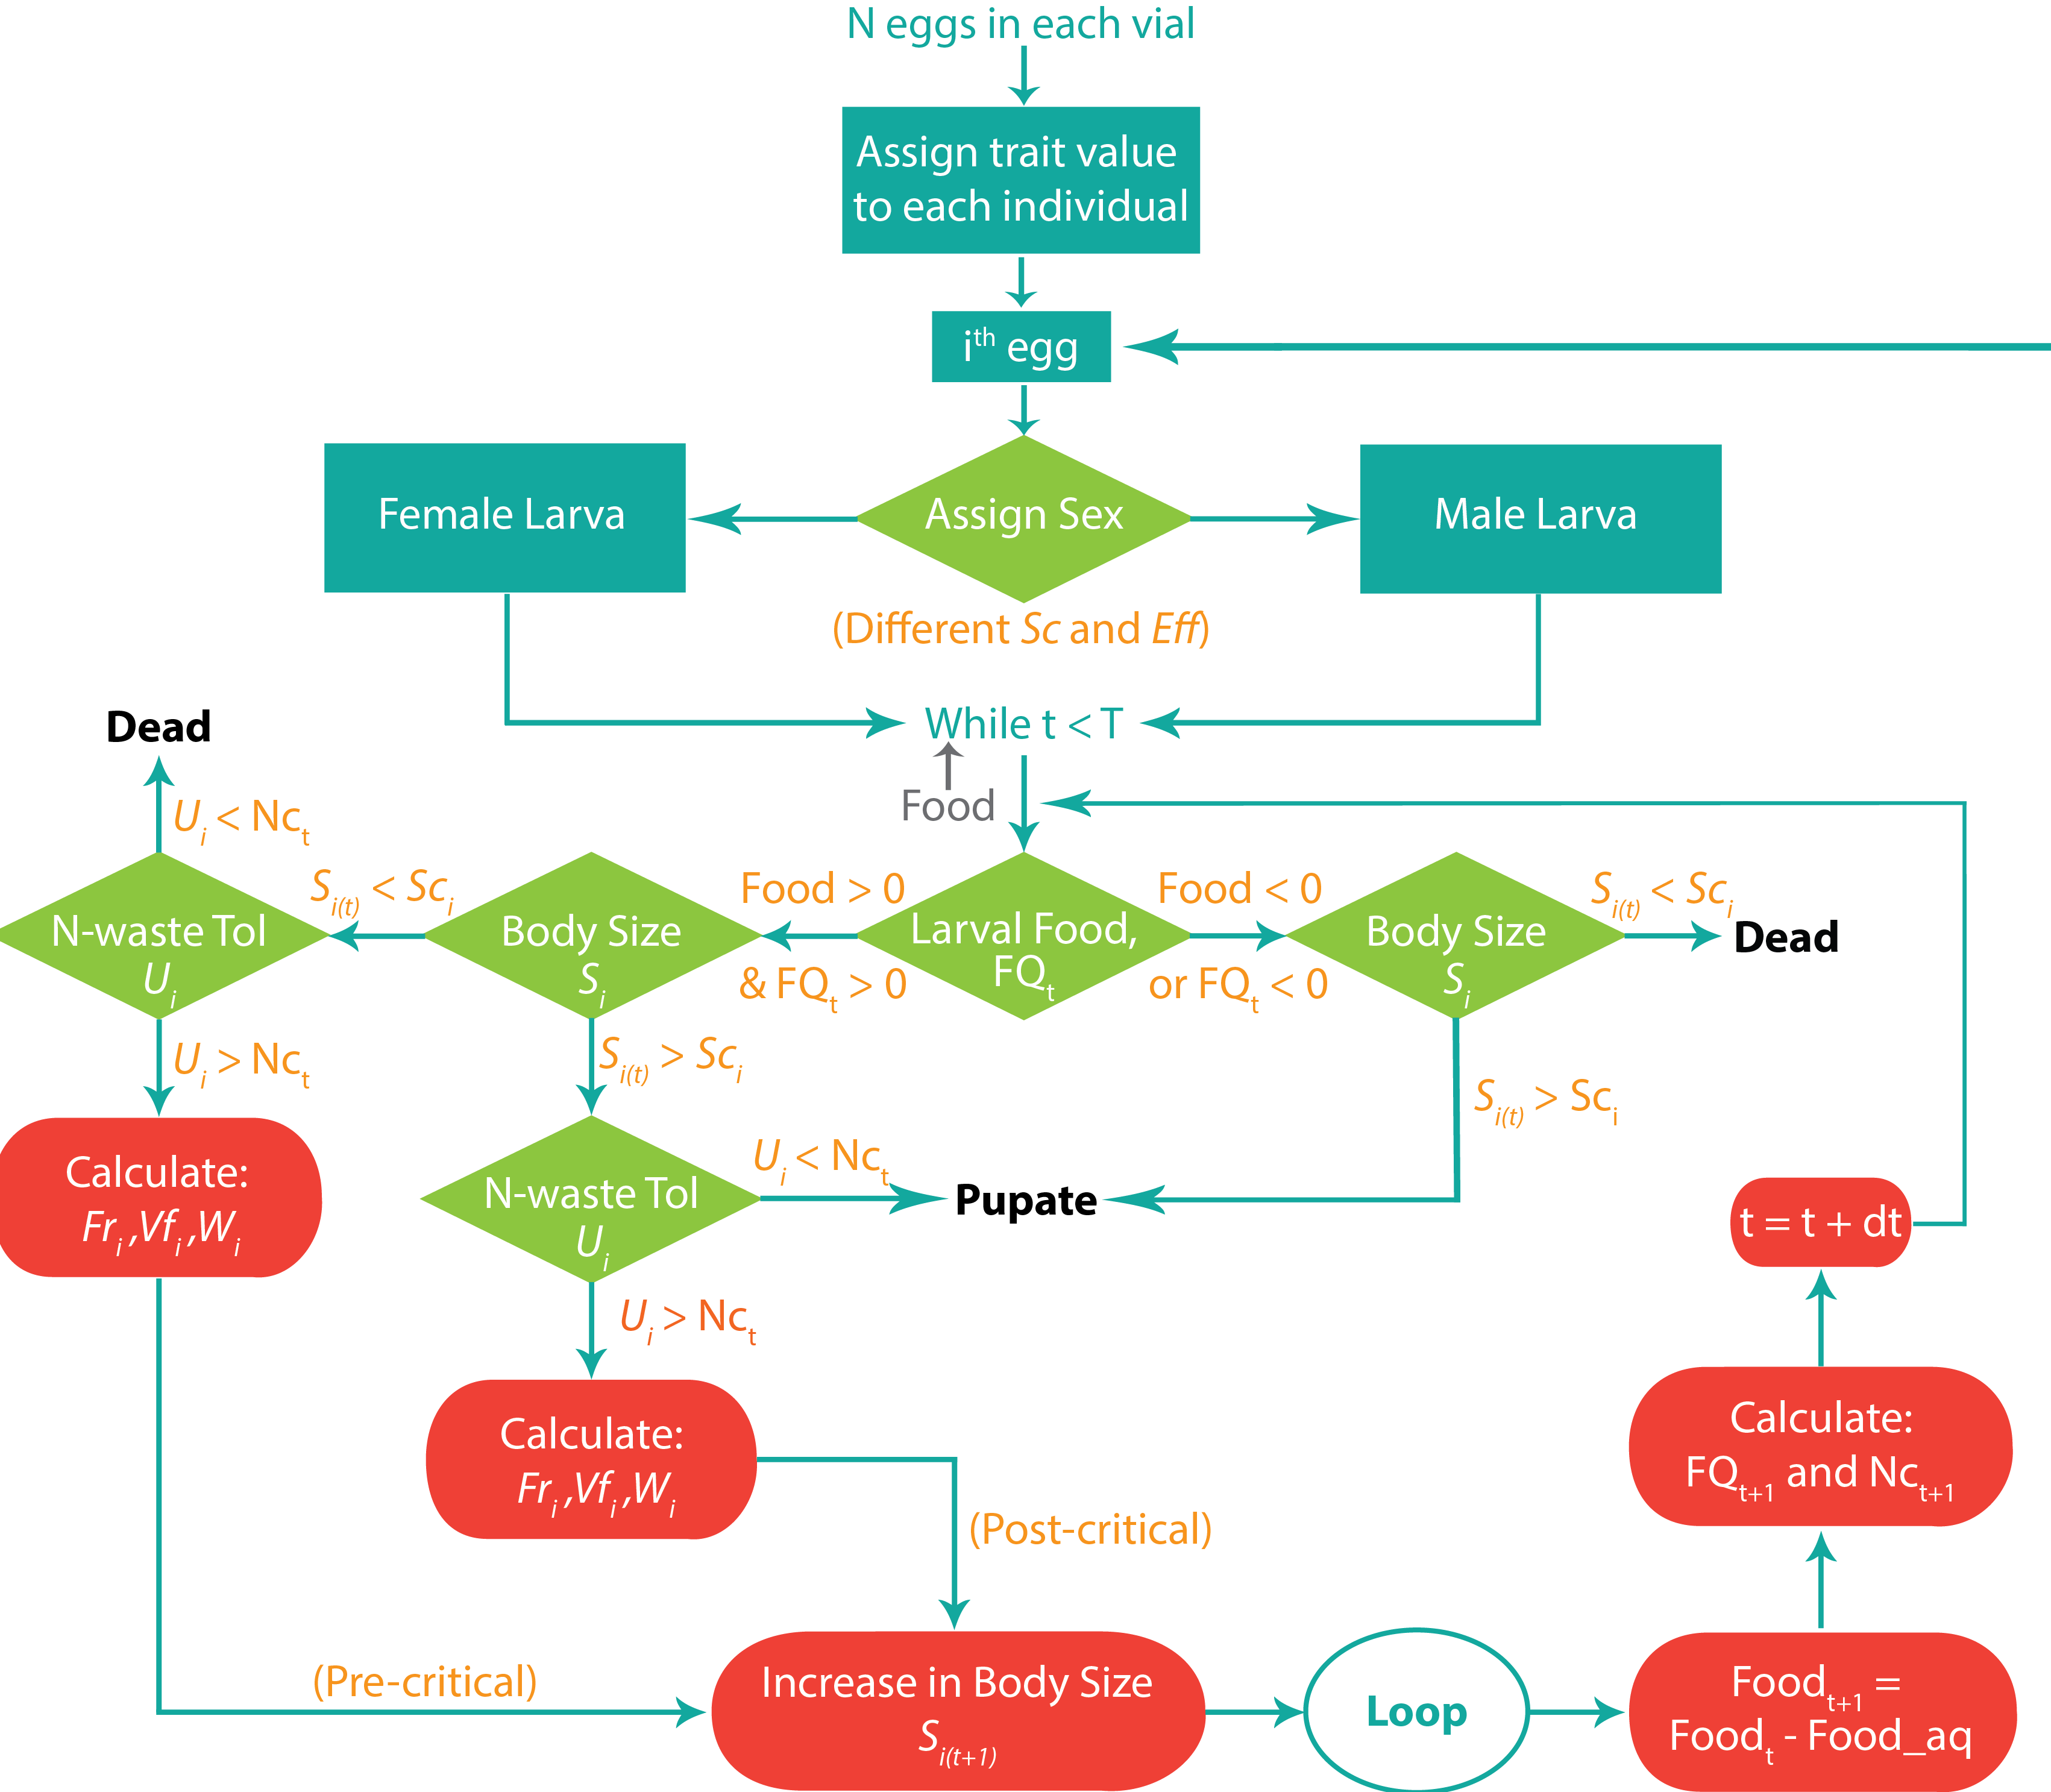
\includegraphics[width=0.8\textwidth]{C2/Figs/larval_model}
  \caption{Flowchart of the larval stage in the model}
  \label{fig:larval_model}
\end{figure}\\
Feeding rate stays constant During post-critical stage. During pre-critical growth Volume of food taken in one bite is taken as constant $V_{f}(pre)$ and during post-critical growth it is $V_{f}(post) = 1.5\cdot V_{f}(pre)$. Food consumed by all larvae at time step $t$ is given as:
\[FoodEaten(t) = \sum_{i}food\_eaten_{i}(t) = \sum_{i}Fr_{i}(t)\cdot V_{f}\]
The increase in body size at time $t$ is $S_{i}(t+1)$ and give as:
\[S_{i}(t+1) = S_{i}(t) + food\_eaten_{i}(t)\cdot \epsilon_{i}\cdot FQ_{fb}(t)\]
Here,\\
$\epsilon_{i}$: Efficiency to convert food eaten into biomass of $i^{th}$ larvae,\\
$FQ_{fb}(t)$: Food quality of the feeding band at time $t$ \\
After feeding and utilizing food consumed at given time step, larva produces nitrogenous waste $waste\_prod_{i}(t)$. This affects the total waste produced by all the larvae after feeding:
\[WasteProd(t) = \sum_{i}waste\_prod_{i} = \sum_{i}[food\_eaten_{i}(t)\cdot (1-\epsilon_{i}\cdot FQ(t))]\]
Based on this waste produced, total waste accumulated till time step $t$ in feeding band and diffusion band is calculated considering $k_{d}$ proportion of waste in the feeding band diffuses into diffusion band at each time step.
\[Waste_{fb}(t+1) = Waste_{fb}(t) + (1-k_{d})\cdot WasteProd(t) + \frac{FoodEaten(t)\cdot Waste_{db}}{dband}\]
\[Waste_{db}(t+1) = Waste_{db}(t) + k_{d}\cdot WasteProd(t) - \frac{FoodEaten(t)\cdot Waste_{db}}{dband}\]
Food quality of the feeding band at time step $t$ is:
\[FQ_{fb}(t) = 1 - \frac{Waste_{fb}(t)}{fband}\]
If $FQ_{fb}(t) \leq 0 $, it means that there is no food available to eat and feeding band contains only nitrogenous waste and larvae stop eating.\\
$k_{d}$ is dependent on the food available in the vial and determines whether waste is diffused into the diffusion band. Its values are assigned at each time step as follows:
\begin{enumerate}[i]
  \item $k_{d}$ is a constant $> 0$ if $food > fband+dband$
  \item $k_{d} = 0$ if $food \leq fband+dband$
\end{enumerate}
Each larva feeds and increase the body size in each time step based on the conditions for food available ($food$), food quality ($FQ(t)$), critical size ($sc_{i}$) and waste tolerance ($u_{i}$) described in fig ~\ref{fig:larval_model}.\\
Values for larval trait parameters obtained from distributions as described in table (ref), were varied and calibrated to obtain survivorship, body size and development time results similar to the empirical results in various larval densities (table no.). These larval trait values represent MB-tpye (control population) larval traits.

\newpage
\section{Feeding Band Dynamics}
Simulations are performed for MB-type larvae to observe the waste build up dynamics in a food vial with different larval densities during larval feeding. In fig ~\ref{fig:waste}, waste build in the feeding band throughout larval feeding at different larval densities is plotted. At low density i.e. 60 eggs / 6 ml food (MB culture), there is very little nitrogenous waste building up due to diffusion and plenty of food available below the feeding band at all time steps unlike at high densities.
\begin{figure}[h]
  \centering
  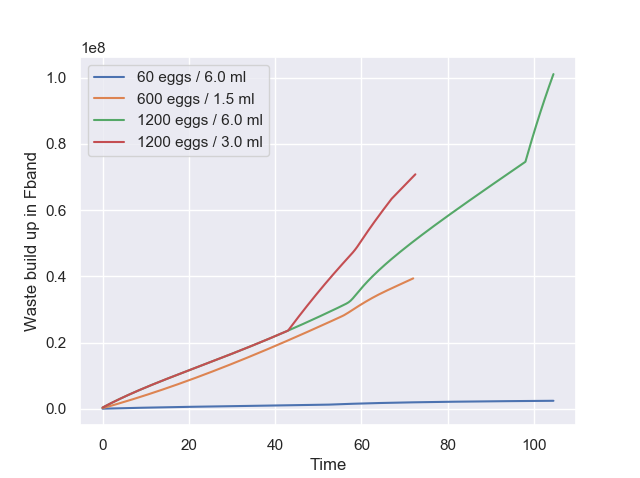
\includegraphics[width=0.8\textwidth]{C2/Figs/waste_build_up}
  \caption{Waste build up in the feeding band}
  \label{fig:waste}
\end{figure}\\
High densities - 600 eggs / 1.5 ml food (MCU culture) and 1200 eggs / 3 ml food (CCU culture) show different patterns of waste build up in the feeding band, even though total larval density is equal. This is due to differences in diffusion pattern in MCU and CCU culture vials. In MCU culture vial, there is very little food available below the feeding band, thus diffusion does not occur and waste build in the feeding band increases gradually. In CCU culture vial, waste build is almost in same qauntity as in MCU culture in earlier stage, even though effective larval density is double (number of larvae per feeding band). This is due to the availablilty of food below feeding band in CCU culture where waste can diffuse. After approx. $40^{th}$ time step, diffusion stops and waste from diffusion band enters feeding band in more quantity, thus giving a sudden increase in the waste build rate. \\ \\
LCU culture vial (1200 eggs in 6 ml food) also shows pattern waste build in the feeding band similar to CCU culture vial, but shows increase in the rate of waste build up at approx. $60^{th}$ time step as there is more food available below the feeding band compared to CCU culture vial. At approx. $100^{th}$ time step in LCU culture vial shows even more increase in the rate of waste build because diffusion band touches the bottom and starts shrinking.
\begin{figure}[h]
  \centering
  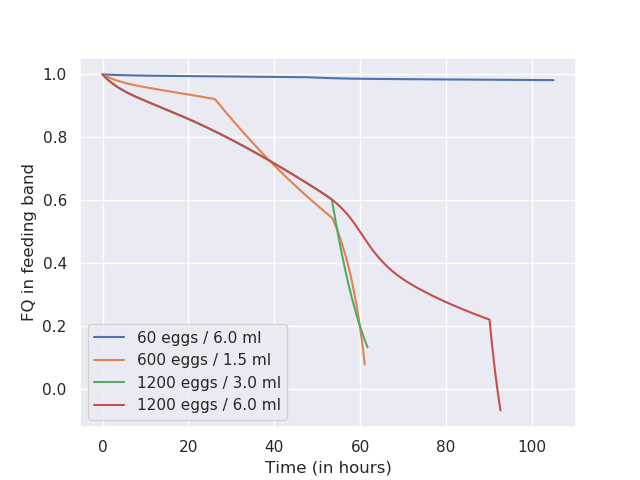
\includegraphics[width=0.8\textwidth]{C2/Figs/fQ}
  \caption{Waste build up in the feeding band}
  \label{fig:fq}
\end{figure}

\pagebreak


  \chapter{Effect of Larval Trait Parameters on Other Life-history Traits}

\section{Initial Feeding Rate and Efficiency}

\section{Initial Feeding Rate and Critical Size}

\section{Efficiency and Critical Size}

\section{Discussion}


\pagebreak
\renewcommand\bibname{{References}}
\bibliography{References}
\bibliographystyle{plain}


  \chapter{Modelling Evolution of Life-history Traits}

\section{Modelling Adult Stage}
After modelling larval stage and calibrating, I developed the model for the adult stage of \textit{Drosophila} life cycle. This includes randomly choosing surviving adults from all replicate larval stage vials, matings, and inheritance of larval trait parameters from parents to offspring. Female is mated once with random male chosen from the adult population with replacement for simplicity. From all the offspring produced, eggs are chosen at random with numbers respective to the crowding environment maintained for the next generation.
\subsection{Fecundity}
After each mating, the number of eggs produced for a female are derived from the fecundity equation based on the model of (ref) Tung S. (year). Fecundity is taken as a function of body size of the female and adult nutrition parameter (the amount of yeast provided). Fecundity of an $i^{th}$ female is given as:
\[Egg_{i} = Nut \cdot x_{2} \cdot \log{(x_{3} \cdot s_{i})}\]
Here, $s_{i}$ = body size of the $i^{th}$ female \\
$Egg_{i}$ = Number of eggs laid by the female in a mating \\
$Nut$ = Adult nutrition i.e. the amount of yeast provided \\
$x_{2}, x_{3}$ = scaling parameters
\subsection{Inheritance}
Larval trait parameters (initial feeding rate, effieciency, waste tolerance and critical size) are inherited from parents to offspring produced by each female using mid-parent value. The mid-parent value i.e. average of mother and father for each larval parameter of offspring as mean is calculated for offspring. This mid-parent value is taken as mean of a normal distribution with fixed standard deviation. The standard deviation in this normal distribution determines the heritibility of the mid-parent value and it is considered to be different for each trait parameter. Trait parameters of the offspring are assigned as:
\[T_{i} \in N(mpv_{T}, \delta_{T})\]
Here, \\
$T_{i}$ = Trait parameter assigned to $i^{th}$ offspring from a mating \\
$mpv_{T}$ = Mid-parent value of of the trait $T$ for a given mating \\
$\delta_{T}$ = Stochasticity in mid-parent value of the trait $T$ \\
$N(mpv, \delta)$ = Normal distribution with $mpv$ as mean and $\delta$ as standard deviation
\section{Effect of Laral Crowding on the Evolution of Life-history Traits}
Using initial values for all parameters given in table (no.), the entire model is simulated for 100 generations with 10 replicates for MB, MCU and CCU cultures. All larval trait parameters are taken from independent distribution and there is no correlation between them. To see how larval trait parameters evolve over time, timeseries for these traits of surviving adult individuals are plotted with 95$\%$ CI. \\\\
Initial feeding rate in high density cultures increase over generations at similar rate but inital feeding rate is higher always in CCU culture always than in MCU culture. In MB culture, being control population, initial feeding rate does not evolve (fig ~\ref{fr}).\\\\
Efficiency show similar trend in high density cultures i.e. it increases over generations at similar rate but is higher always in CCU culture always than in MCU culture. In MB culture, being control population, efficiency does not evolve (fig ~\ref{eff}).
\newpage
\begin{figure}
  \centering
  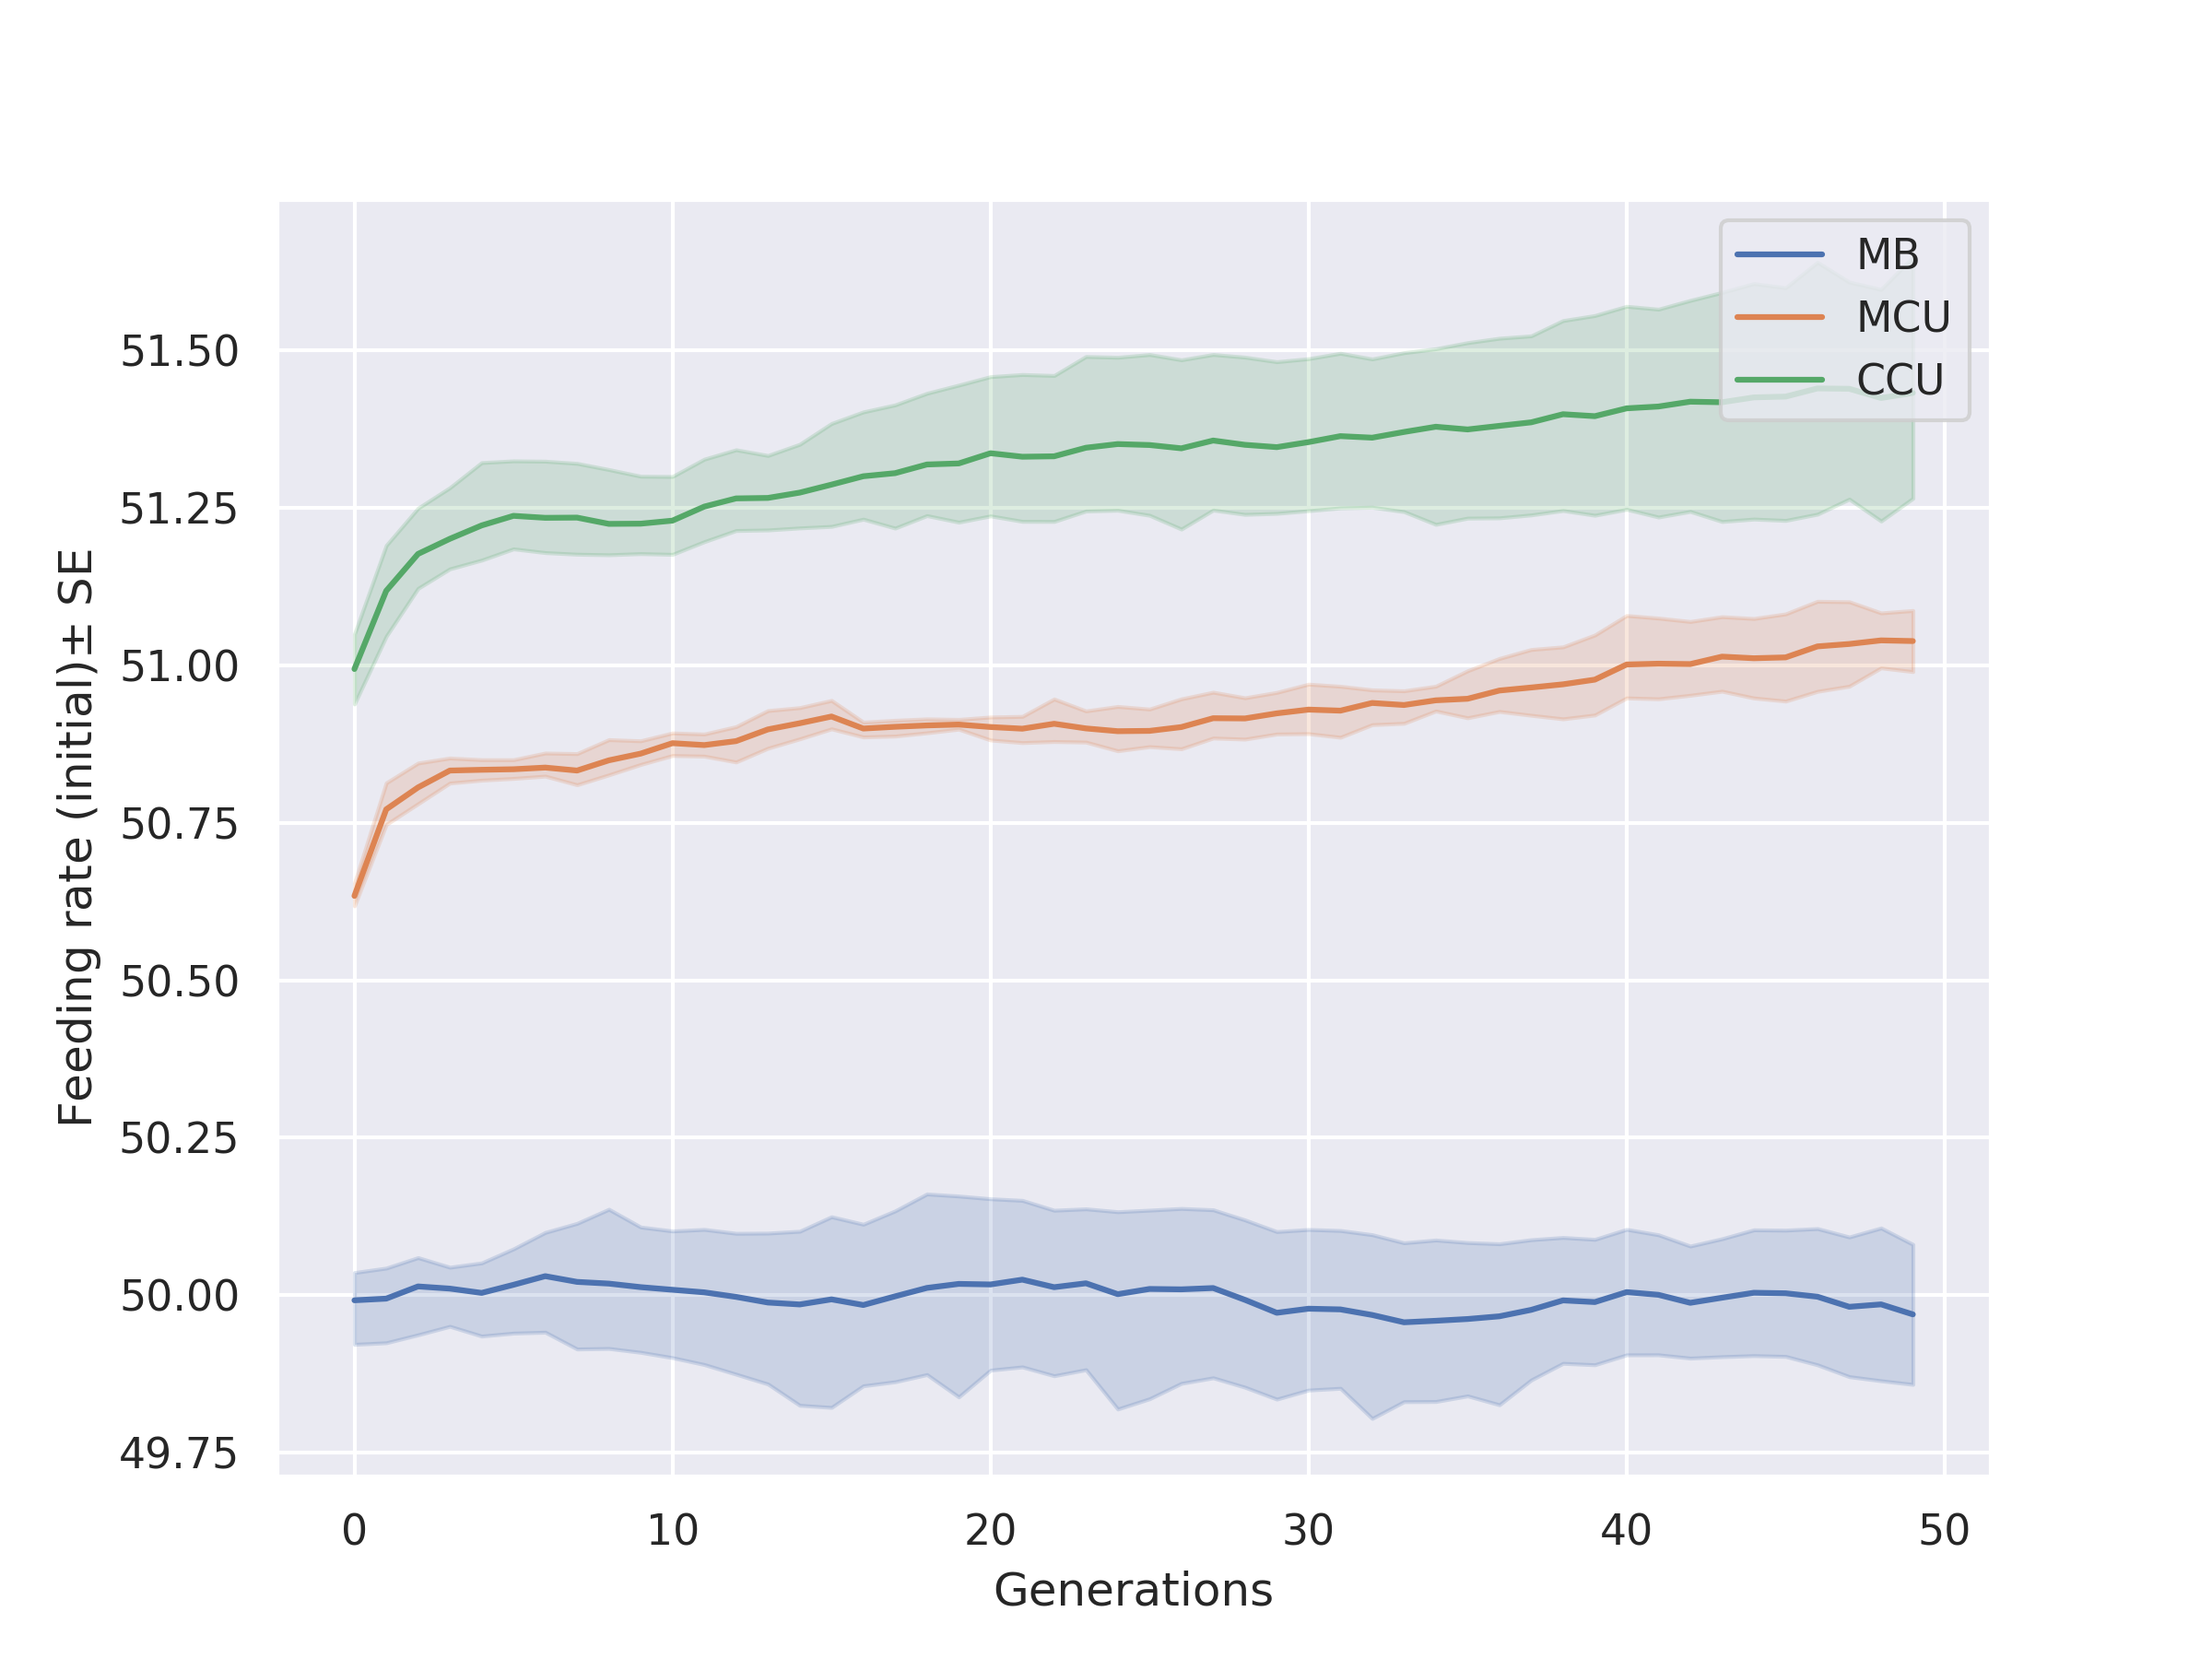
\includegraphics[width=0.9\textwidth]{C4/Figs/fr}
  \caption{Timeseries for initial feeding rate}
  \label{fr}
  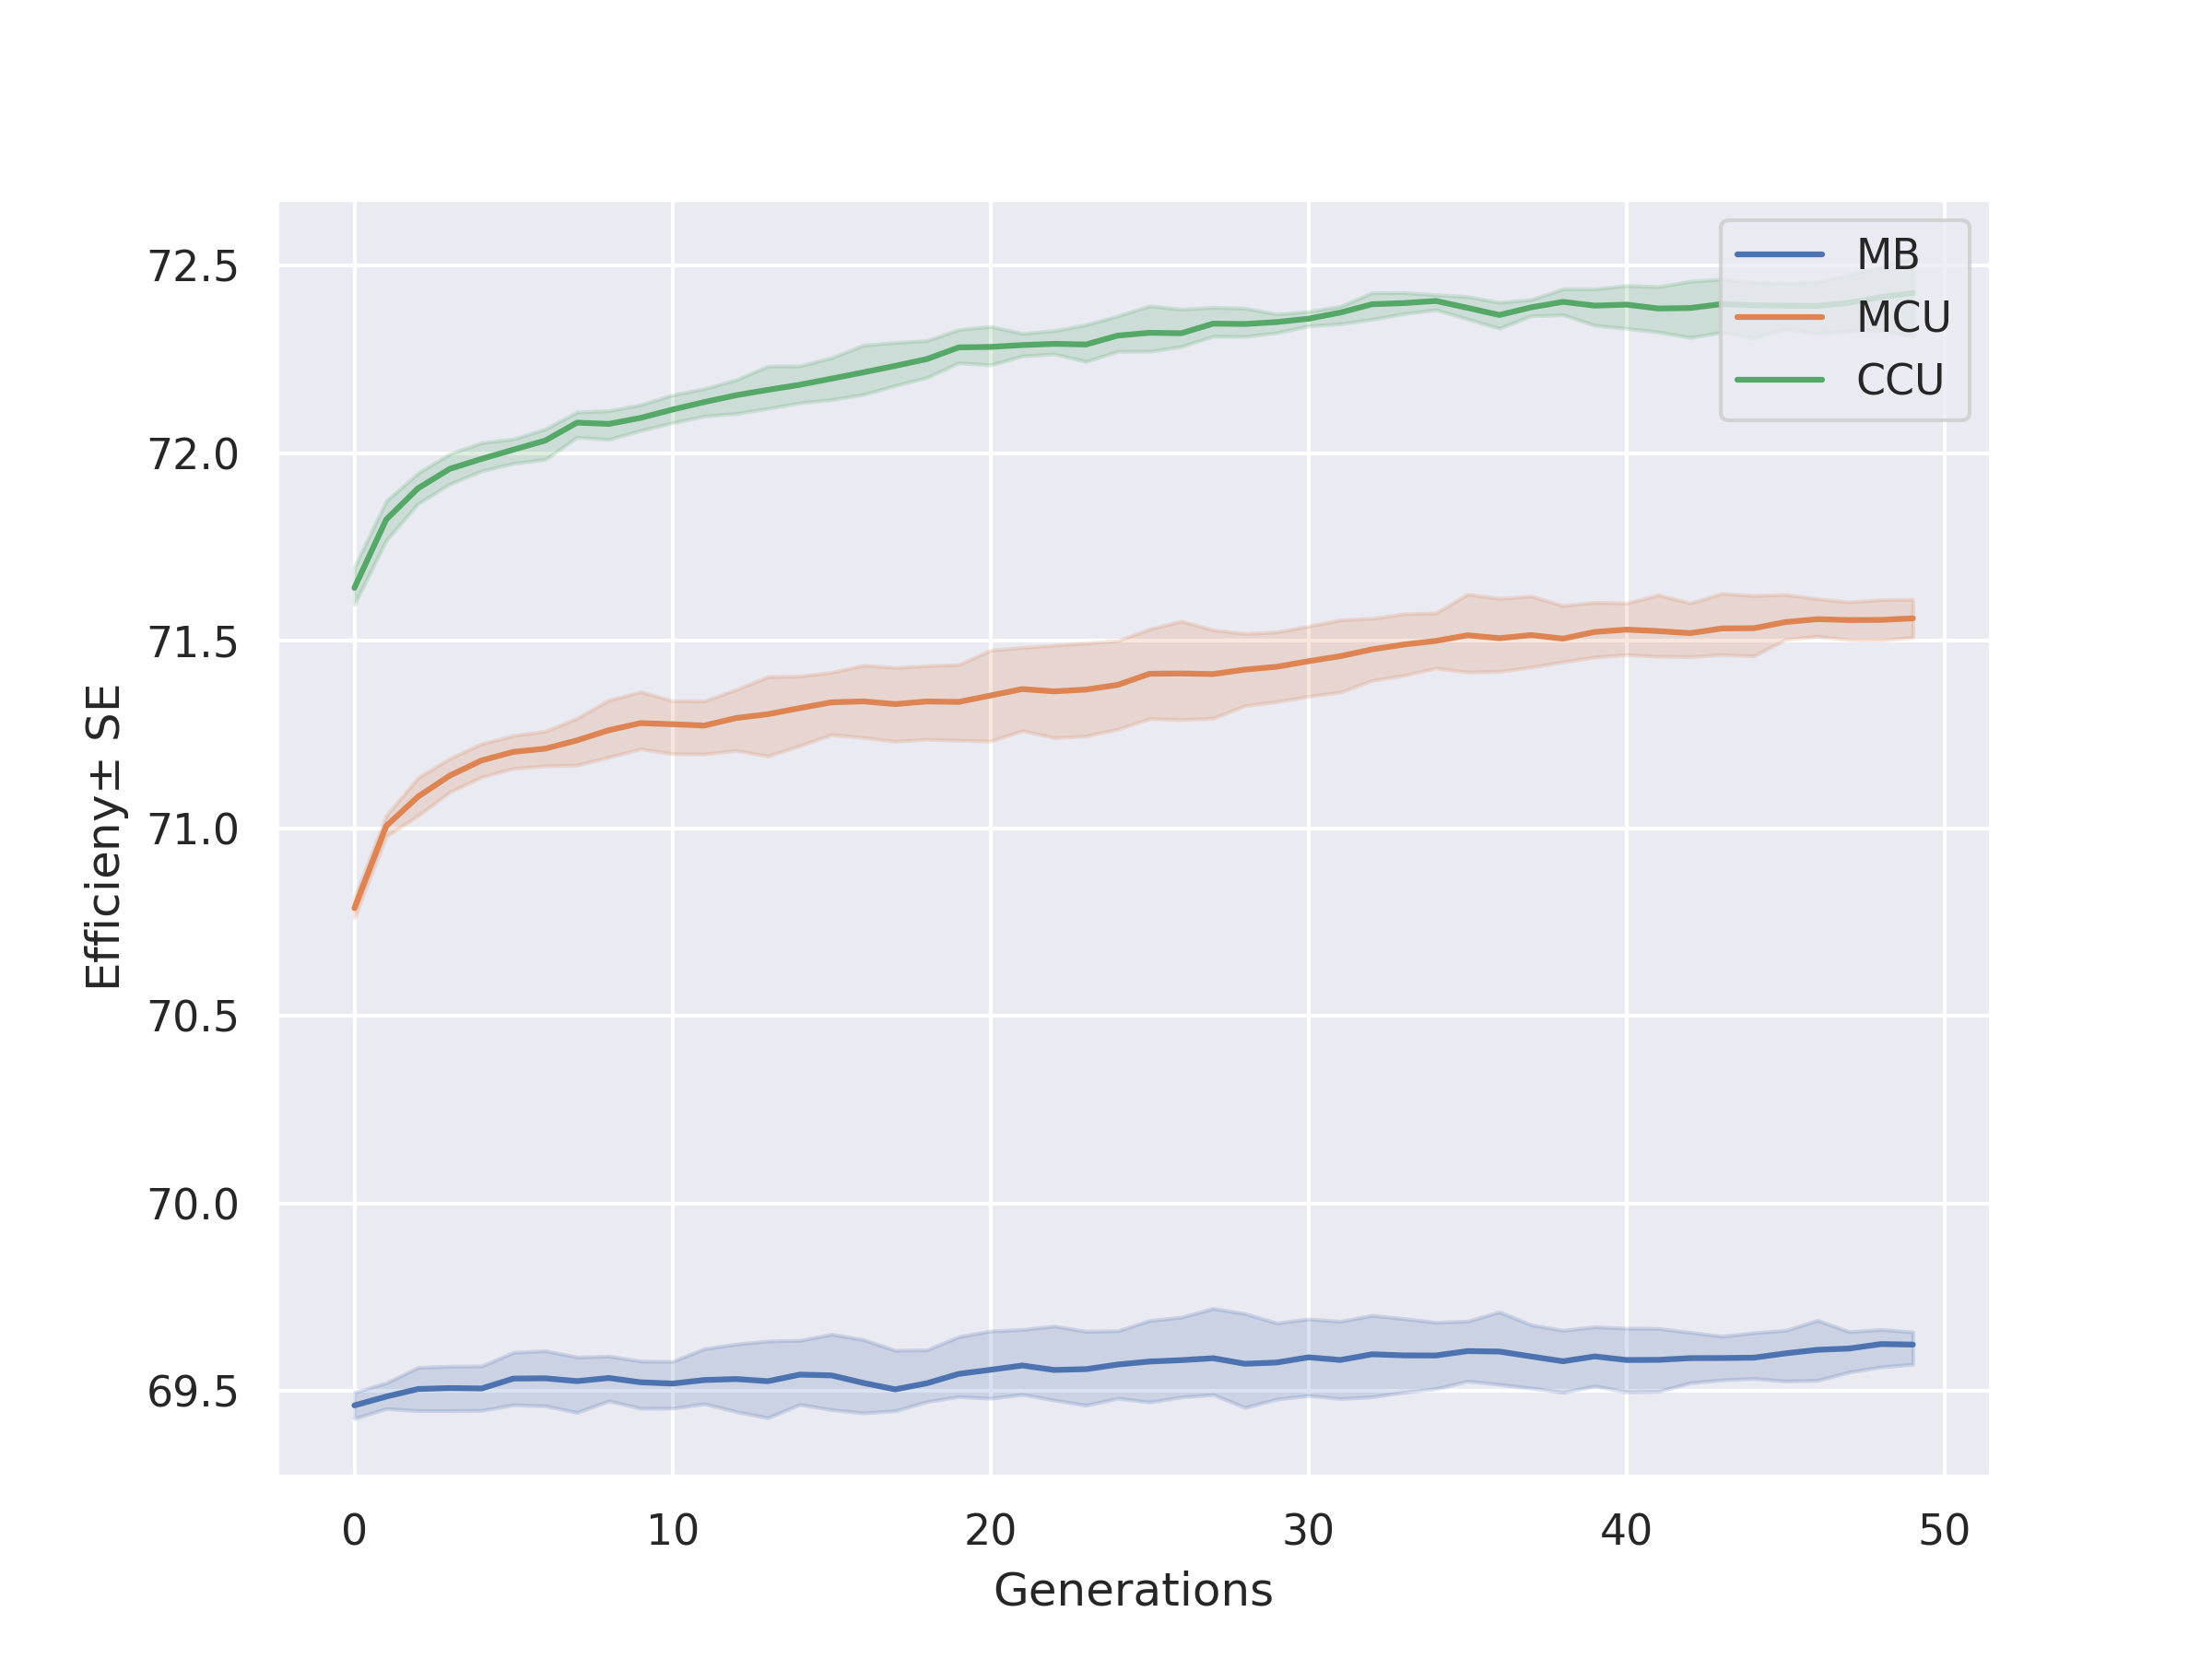
\includegraphics[width=0.9\textwidth]{C4/Figs/eff}
  \caption{Timeseries for initial efficiency}
  \label{eff}
\end{figure}
\newpage
Critical size in high density cultures decreases at the same rate but critical size in CCU culture is always lower than in MCU culture. In MB culture, critical size does not change over generations (fig ~\ref{mc}). \\\\
Waste tolerance does not evolve in all of the culture populations since there is no significant decrease/increase in waste tolerance value (fig ~\ref{wtol}).
\newpage
\begin{figure}[h]
  \centering
  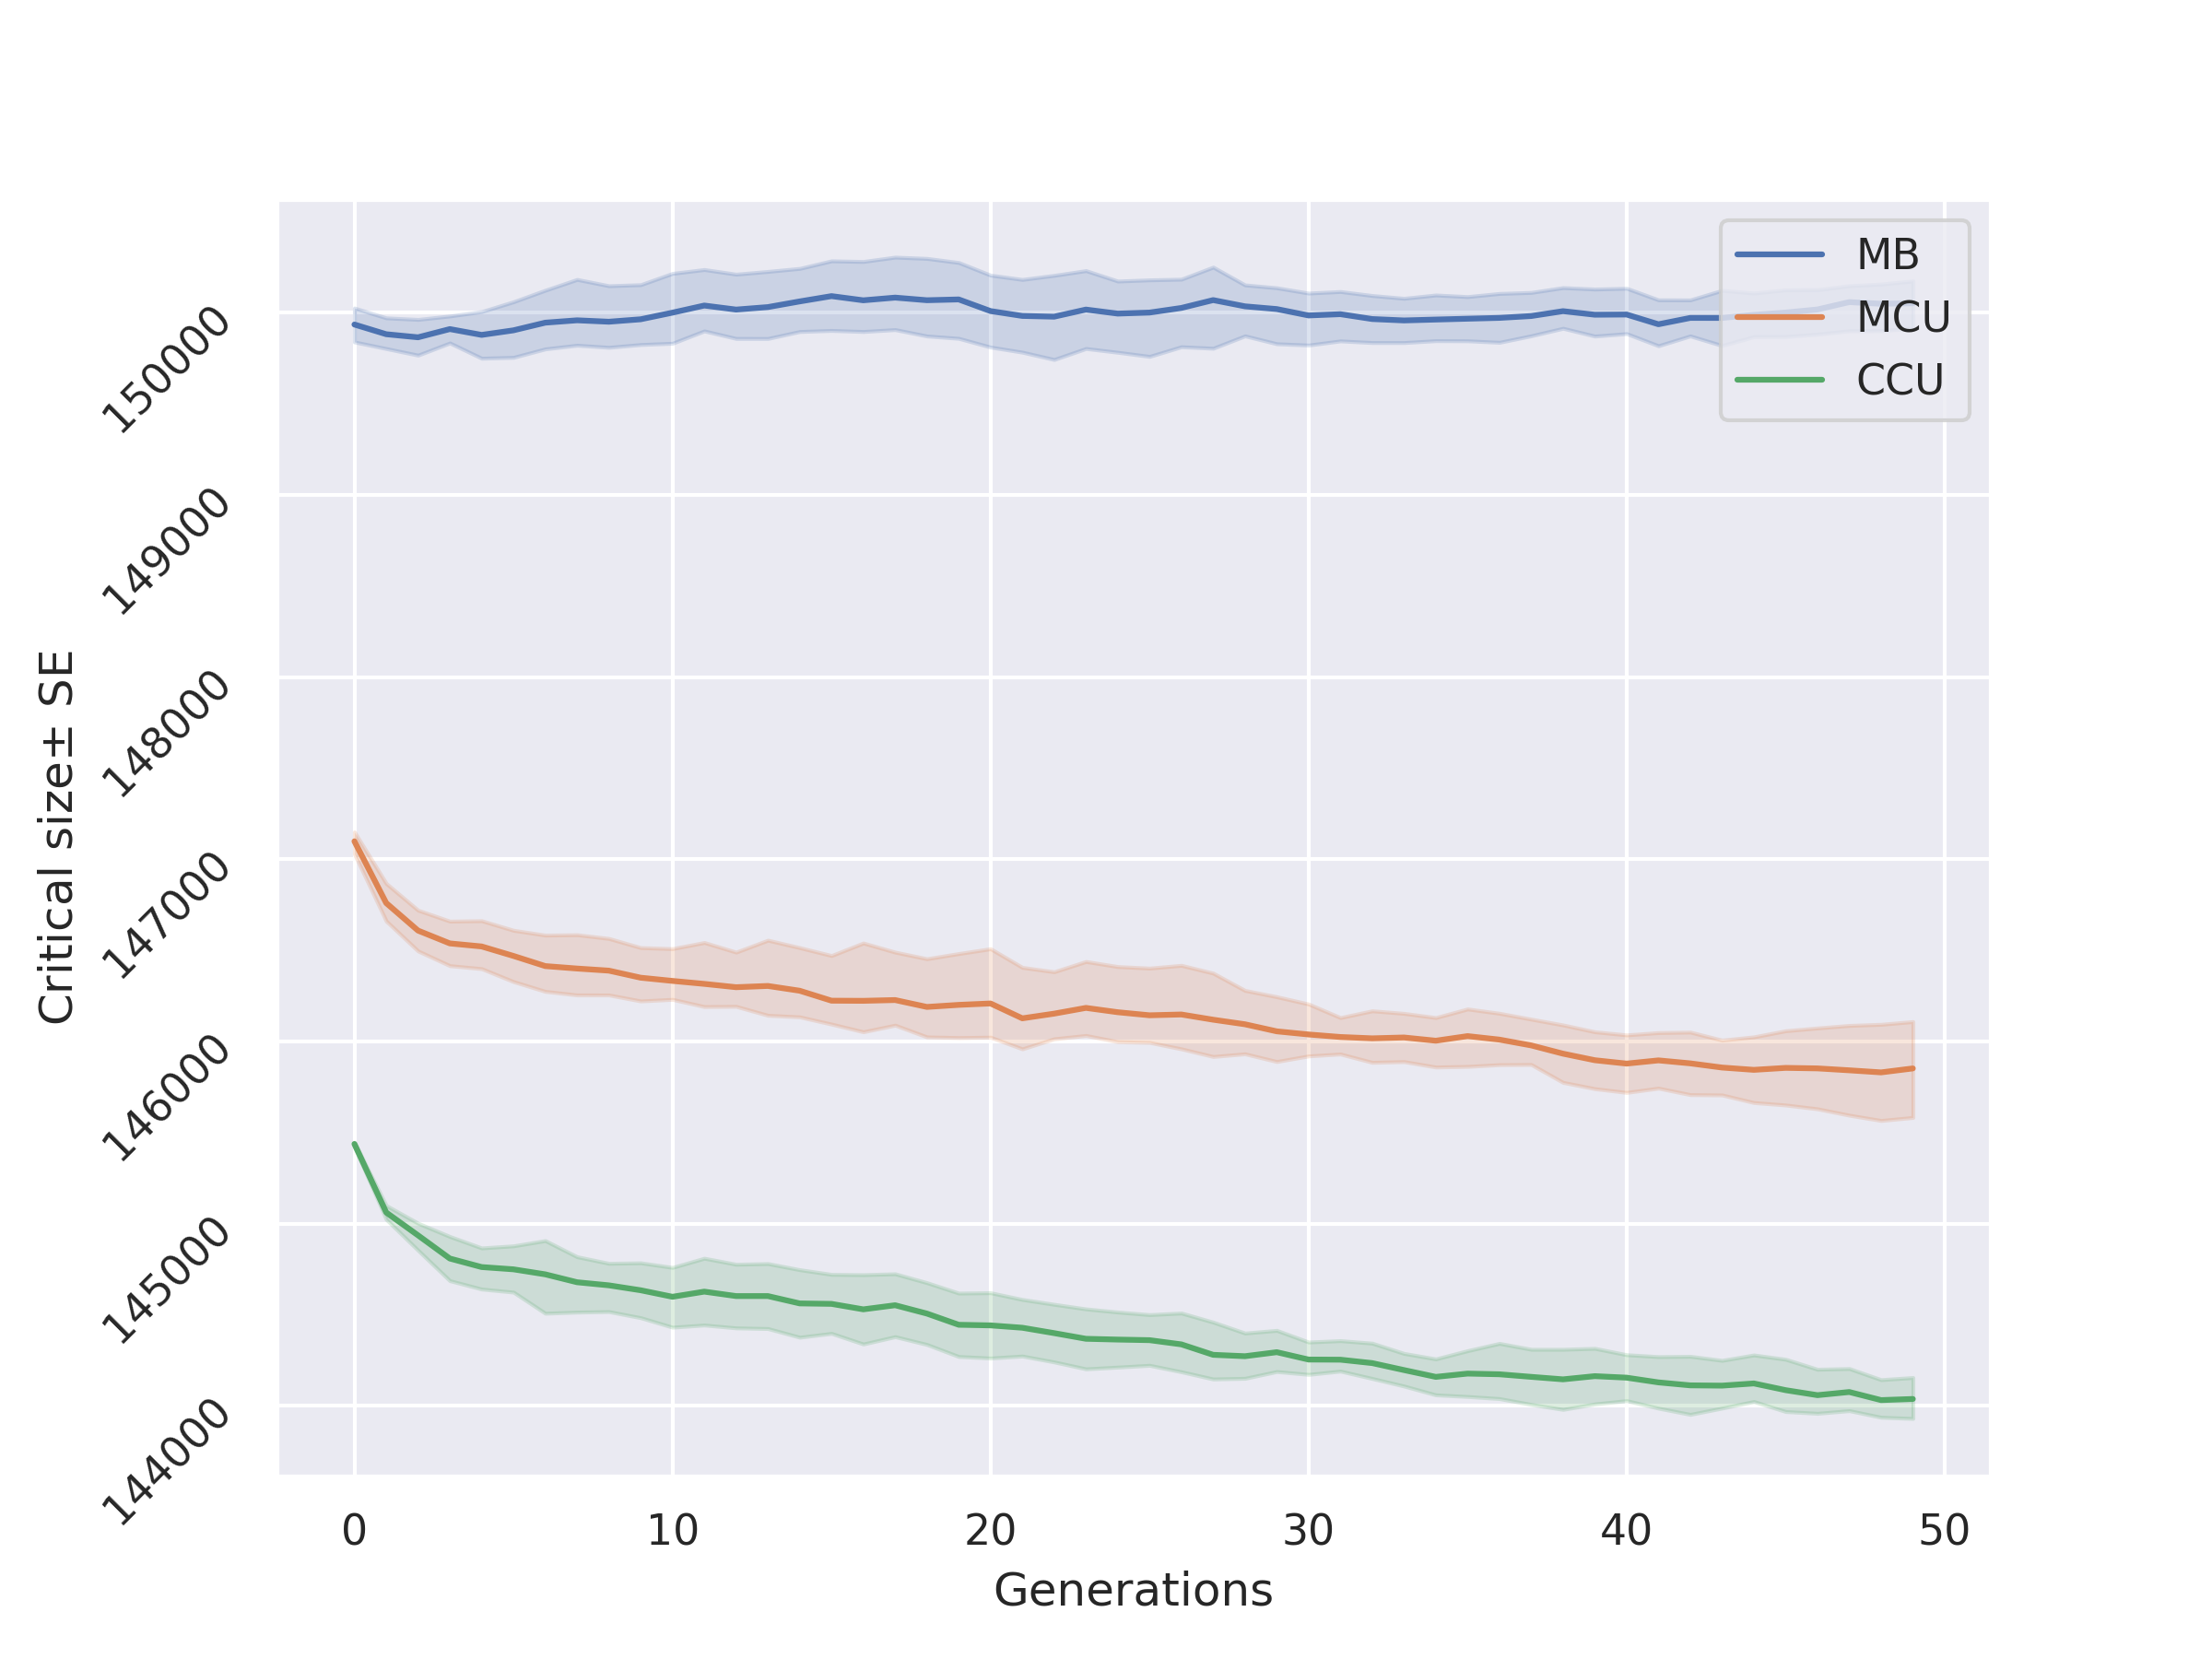
\includegraphics[width=0.9\textwidth]{C4/Figs/mc}
  \caption{Timeseries for initial critical size}
  \label{mc}
  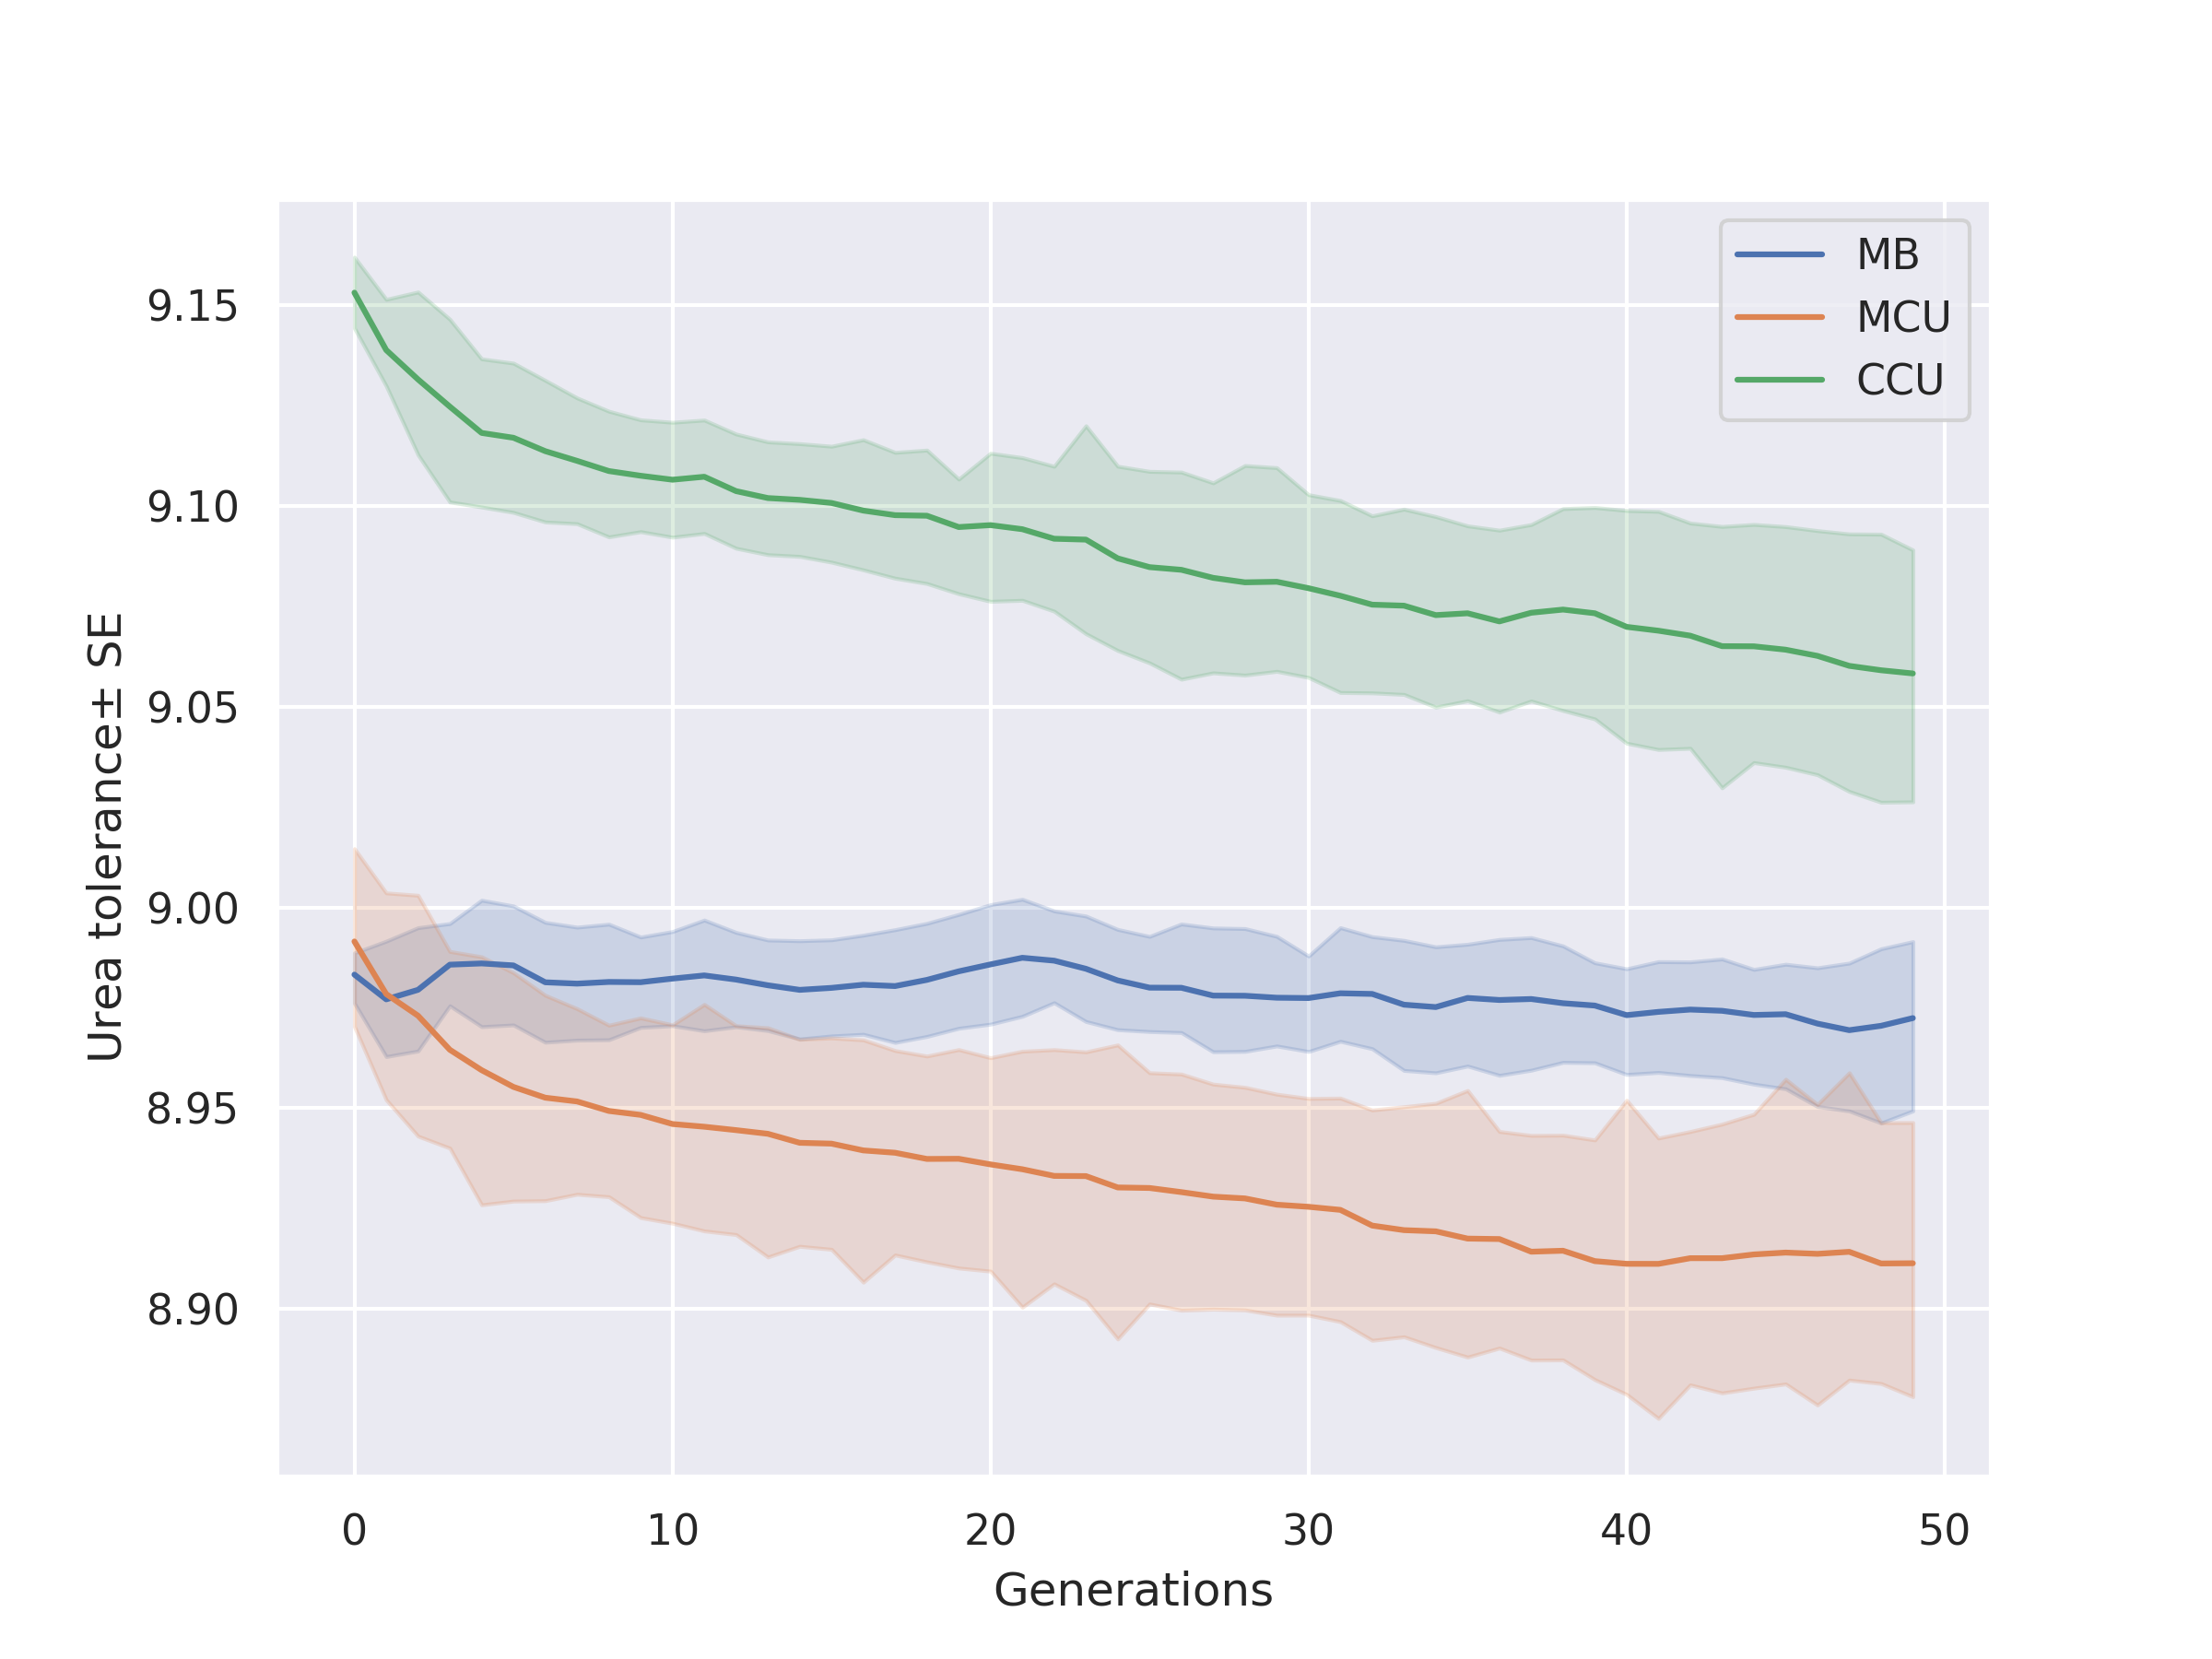
\includegraphics[width=0.9\textwidth]{C4/Figs/wtol}
  \caption{Timeseries for initial waste tolerance}
  \label{wtol}
\end{figure}
\newpage
\section{Effects of Variation on the Evolution of Larval Trait Parameters}
The source of variation in the model comes from the initial variation in the larval trait parameters, given as certain standard deviation in the respective initial distribution as well as from the heritibility of the mid-parent value during the inheritance of the larval trait parameters. The simulations show how these sources of variations play an important role in determining the evolutionary routes taken to acheive greater competitive ability by having maximum survivorship.
\subsection{Variation in the Initial Distribution of Larval Trait Parameters}
When timeseries are plotted for the larval trait parameters, the variation in the initial distribution of these trait parameters determine the maxima that can be achieved to increase the fitness. From fig(a), fig(b) and fig(c), it is seen that differences in variation of these trait values, maxima reached are different with similar initial mean trait values. If the initial variation in efficiency is very high compared initial variation in feeding rate, then feeding rate does not reach higher feeding rate after few generations unlike of the timeseries simulations performed with lower initial variation in the efficiency. Depending on the initial variation in each trait separately, traits can evolve differently, since these trait parameters interact with each other to give complex phenotypes suxh as body size, time to rach critical size and survivorship.
\subsection{Heritibility in Mid-parent Value}

%\section{Discussion}

\pagebreak
%\renewcommand\bibname{{References}}
\bibliography{References}
\bibliographystyle{plain}


  \chapter{Introducing Correlations in Larval Trait Parameters}

\section{Distribution of Laral Traits with Development Time}

\section{Effects of Negative Correlation between Feeding Rate and Efficiency}

\section{Discussion}

\pagebreak
\renewcommand\bibname{{References}}
\bibliography{References}
\bibliographystyle{plain}


  \setlength\bibitemsep{\baselineskip}
  %\addcontentsline{toc}{chapter}{References}
  %\printbibliography[title=References]

  \renewcommand{\baselinestretch}{1.5}
  \appendix
  \chapter{Code}
This appendix contains code written for larval stage and adult stage in the model. All code is written in Python 3.7 (\citeauthor{WelcomePythonOrg}, \url{www.python.org}).
\lstset{
  columns=fullflexible,
  frame=single,
  breaklines=true,
  postbreak=\mbox{{$\hookrightarrow$}\space},
}
\lstdefinestyle{mystyle}{
    backgroundcolor=\color{backcolour},
    commentstyle=\color{codegreen},
    keywordstyle=\color{magenta},
    numberstyle=\tiny\color{codegray},
    stringstyle=\color{codepurple},
    basicstyle=\ttfamily\footnotesize,
    breakatwhitespace=false,
    breaklines=true,
    captionpos=b,
    keepspaces=true,
    numbers=left,
    numbersep=5pt,
    showspaces=false,
    showstringspaces=false,
    showtabs=false,
    tabsize=2
}
\lstset{style=mystyle}

\section{Larval Stage}
\lstinputlisting[language=Python]{CA1/Scripts/larva_index_base.py}
\section{Adult Stage}
\lstinputlisting[language=Python]{CA1/Scripts/timeseries.py}
The entire code is on the following Github repository:\\
\url{https://github.com/ElY0da/Thesis_code.git}
\begin{figure}[h]
  \centering
  
\includegraphics[width=0.3\textwidth]{CA1/github_code}
  \caption{QR code for Github repository containing all codes}
\end{figure}
\clearpage


\end{document}
